\documentclass[fleqn,10pt]{physiome}
% Use option lineno for line numbers 
\usepackage{subfigure}
\articletype{Retrospective}
%% Choose from Original, Retrospective, Review, Letter

\title{Reproducibility study to simulate a chain of collapsible contracting lymphangions with progressive valve closure}

\author[1][t.jayathungage-don@auckland.ac.nz]{Tharanga D. Jayathungage Don}
\author[1]{Alireza Sharifzadeh-Kermani}
\author[1]{Soroush Safaei}
\author[2]{Peter S. Russell}
\author[2]{Anthony R. J. Phillips}
\author[1]{Hayley M. Reynolds}
\affil[1]{Auckland Bioengineering Institute, University of Auckland, New Zealand}
\affil[2]{Department of Surgery, Faculty of Medical and Health Sciences, Surgical and Translational Research Centre, University of Auckland, New Zealand}

%% The following lines can be omitted when submitting;
%% information will be added by editors
%% The following lines can be omitted when submitting;
%% information will be added by editors
\publicationdate{14 May 2024}
\editor{David P. Nickerson}
\curator{Shelley Fong}
\submitteddate{10 Nov 2023}
\accepteddate{13 May 2024}
\citethisas{Jayathungage Don et al. (2024)\\Reproducibility study to simulate a chain of
collapsible contracting lymphangions with progressive valve closure. Physiome.}{10.36903/physiome.25814500}
\begin{document}

\maketitle

\begin{abstract}
This paper presents a reproduced computational model of lymphatic collecting vessels. The model was originally introduced by \cite{bertram2011simulation}, and comprises a series of contractile segments, known as lymphangions, interconnected by secondary lymphatic valves. The model focused on elucidating the pumping behavior of contracting lymphangions and deriving pump-characteristic curves, by incorporating pressure-dependent valve resistance, passive elasticity, and active contraction terms in multiple lymphangions. The original model was implemented and solved using MATLAB software. In our work, we reproduce \citeauthor{bertram2011simulation}'s original model within the CellML framework, and present the results.  

\end{abstract}

\keywords{CellML, OpenCOR, computational model, lymphatic vessels, lymphangion, valve}

\primarypubs[10.36903/physiome.25814500]{sample}{bertram2011simulation}

\section{Introduction}
The primary paper of \cite{bertram2011simulation} introduced a model comprising a series of lymphangions connected via inter-lymphangion valves. The objective of their study was to take the first step toward developing a comprehensive model of the lymphatic system. The original contribution of \cite{bertram2011simulation}'s work lies in incorporating a pressure-dependent valve resistance and the consideration of the constitutive equation of the vessel wall, including passive elasticity and active contraction terms.

The model of \cite{bertram2011simulation} played a significant role in collecting lymphatic modelling, and subsequent studies \citep{Bertram2014_b2, Bertram2016, Bertram2017} have improved and validated it by using ex-vivo experimental data published in later years \citep{Davis2011, Davis2012}. Over the last decade, there has been a surge of interest in lymphatic-related research \citep{don2023review}. Despite this, the lymphatic system remains one of the least explored areas in biomedical research. Freely available and open-source reproducible lymphatic models aim to advance lymphatic research.

\section{Model description}
\begin{figure}
    \centering
    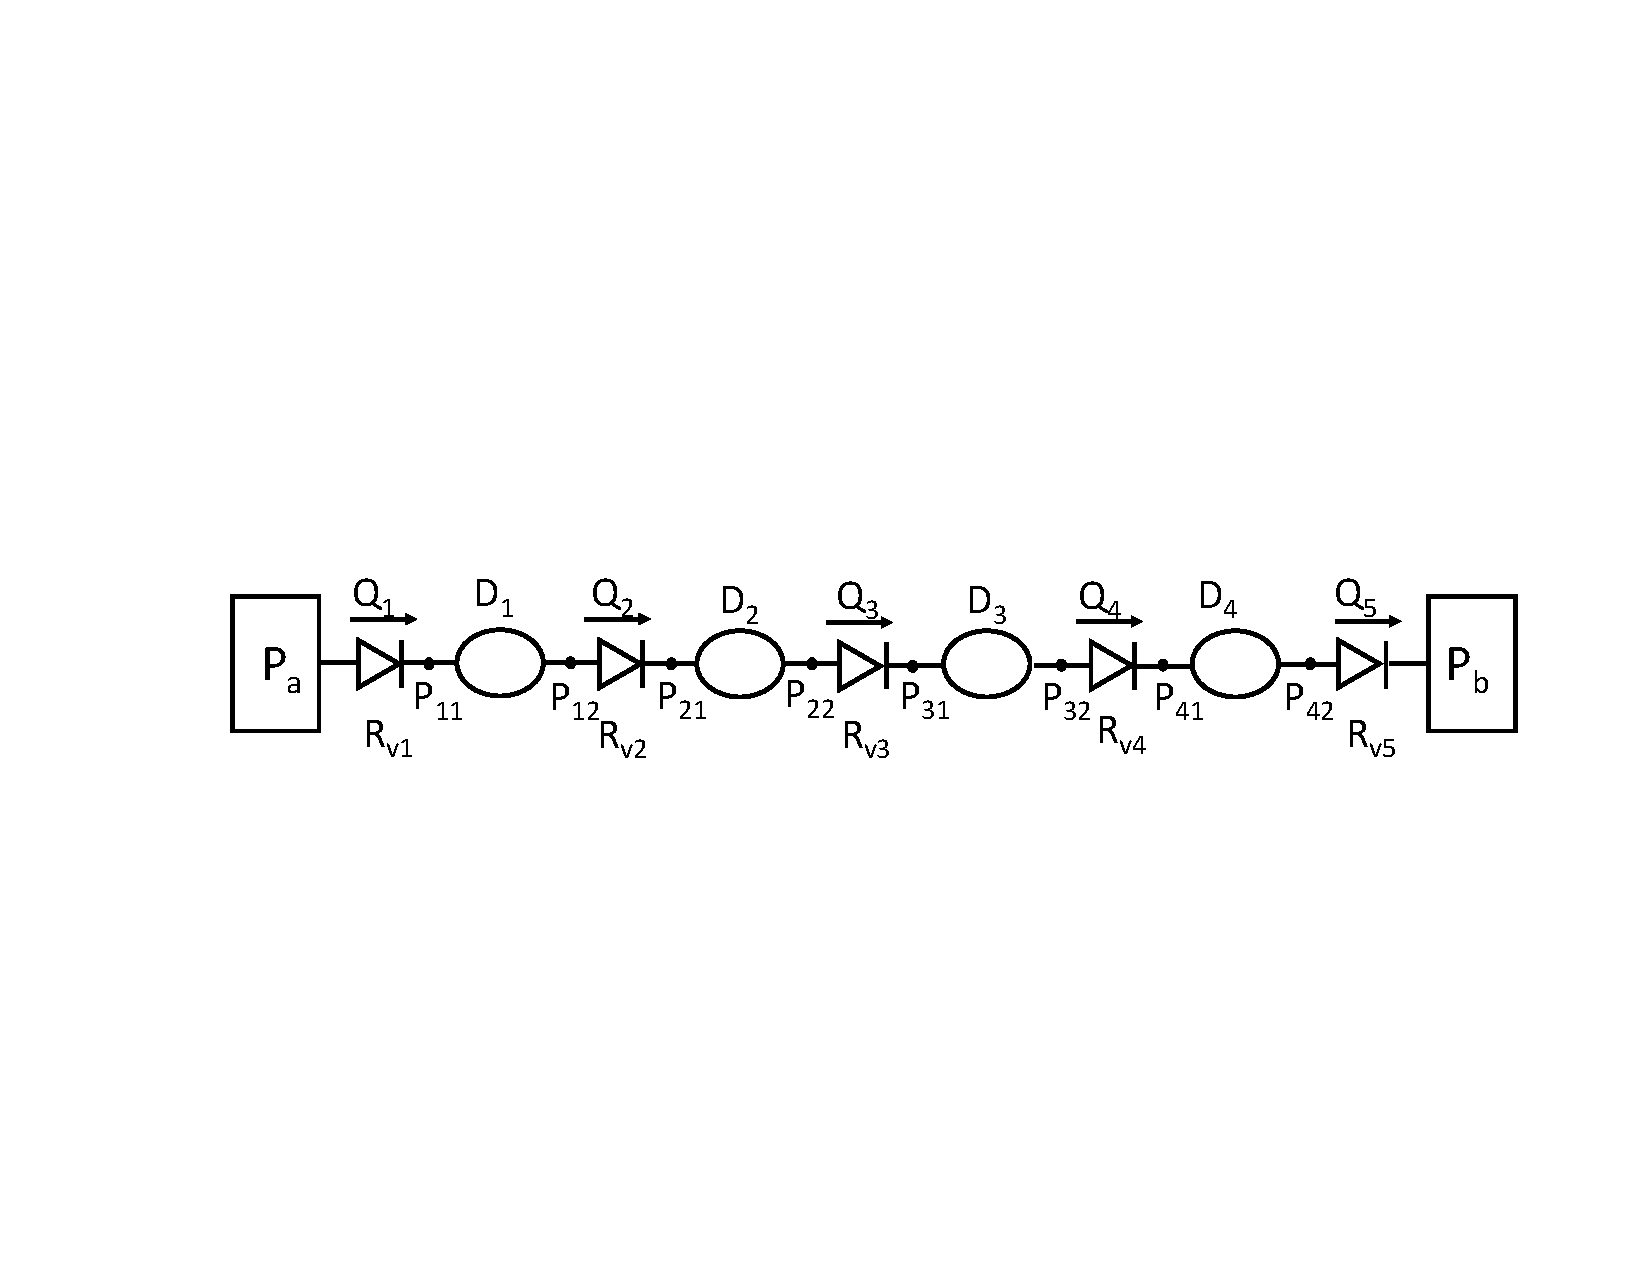
\includegraphics[trim=3.10cm 7.0cm 0.10cm 7.0cm, clip=true, totalheight=0.2\textheight,  ]{Lymphangion_model.pdf}
    \caption{A schematic diagram of the lymphangion-chain model displays the contractile vessel segments, each characterized by its diameter (D). These segments are separated by one-way flow valves, with the flow rate denoted as Q, and the flow resistance as $R_{V}$. At each connection point that links these components, effectively covering both the upstream and downstream ends of each segment, the pressure (P) is explicitly defined. P$_{a}$ and $P_{b}$ represent constant pressure values at the boundaries. }
    \label{fig:schematic}
\end{figure}

Figure \ref{fig:schematic} shows a schematic diagram of a chain of contractile vessel segments linked via secondary valves. Both ends are connected to constant pressure boundary conditions, P$_{a}$ and $P_{b}$. The chain is subjected to uniform external pressure, P$_{e}$. The pressure-dependent valve resistance is implemented using a sigmoidal function. Flow inside the vessels is modelled using the Poiseuille flow equation. Additionally, the force balance equation for the vessel walls includes both passive and active contractile components. The resultant ordinary differential equation (ODE) system is non-linear. The parameter values and boundary conditions are listed in Table 1 and Figures 4 and 5 in the captions of the primary paper. 

The mathematical model was implemented within the open-source, extensible markup language (XML)-based CellML modeling environment. CellML is widely utilized for representing mathematical models in the field of biology, employing ODE and algebraic equations (\citealp{cuellar2003overview}). All simulations were executed using OpenCOR (Version 0.7) as the simulation platform (\citealp{garny2015opencor}). The original CellML file and all the associated code can be accessed by following this link within the PMR: \url{https://models.physiomeproject.org/workspace/b44}.


\section{Computational Simulation}

The Bertram2011.cellml file contains the necessary code to execute the simulation. The simulation, conducted over 100 seconds with a time step of 0.0001 seconds, was completed in approximately 4.5 seconds of wall clock time. The CVODE solver was employed, and the simulation was executed on a Windows desktop computer equipped with an Intel Core i7 10th generation CPU. Additionally, the following solver settings were applied: a maximum step of 0.0001 and a total of 5 $\times$10$^{5}$ steps.


OpenCOR offers the capability to export results in CSV format. When exporting the CSV file for a specific set of parameters and boundary conditions, the following data must be selected from the drop-down menu: time, Q1 to Q5 (Valve\_1 to Valve\_5), D (Vessels\_1 to Vessels\_4), Mfunc\_1 to Mfunc\_4, P11, P12, P21, P22, P31, P32, P41, and P42 values. Subsequently, MATLAB scripts (\texttt{PlotGenerator\_figure\_4.m} and \texttt{PlotGenerator\_figure\_5.m}), available in the PMR, were utilized to generate plots after reading the CSV result files. Importantly, the column names of the output CSV file must be changed based on the defined variable names in the \texttt{PlotGenerator.m} files.

The column names should be adjusted as follows:
\begin{itemize}
    \item Rename "environment | time (second)" to "T"
    \item Rename "Valve\_1 | Q1 (ml\_per\_s)-Valve\_5 | Q5 (ml\_per\_s)" to "Q1-Q5"
     \item Rename "Vessel\_1 | D (cm)-Vessel\_4 | D (cm)" to "D1-D4"
    \item Rename "Vessel\_1 | Mfunc\_1 (dyn\_per\_cm2)-Vessel\_4 | Mfunc\_4 (dyn\_per\_cm2)" to "M1-M4"
    \item Remove vessel numbers and units from pressure values (e.g., "Vessel\_1 | P11 (dyn\_per\_cm2)" becomes "P11").
\end{itemize}

Save the CSV file as "Bertram\_2011\_Data\_figure4/5.csv". Then, running the MATLAB script will produce the correct figures.



\section{Model results}

The simulated results for a chain of four lymphangions against two sets of prescribed pressures, P$_{a}$=2275 dyn cm$^{-2}$ P$_{b}$=2875 dyn cm$^{-2}$ and P$_{a}$=2275 dyn cm$^{-2}$ P$_{b}$=2375 dyn cm$^{-2}$, prescribed in the original work are demonstrated here. Figures \ref{fig:reproduced_1} and  \ref{fig:reproduced_2} show active tension, diameter variation, pressure values at different locations, and flow rates for each lymphangions. 
Figures \ref{fig:reproduced_1} and \ref{fig:reproduced_2} correspond to Figures 4 and 5, respectively, in the primary paper. We employed the exact parameter values as specified in the primary paper. The parameter values used in the CellML model for Figures \ref{fig:reproduced_1} and \ref{fig:reproduced_2} are presented in Table \ref{table_para1}.
\begin{figure}[p]\centering
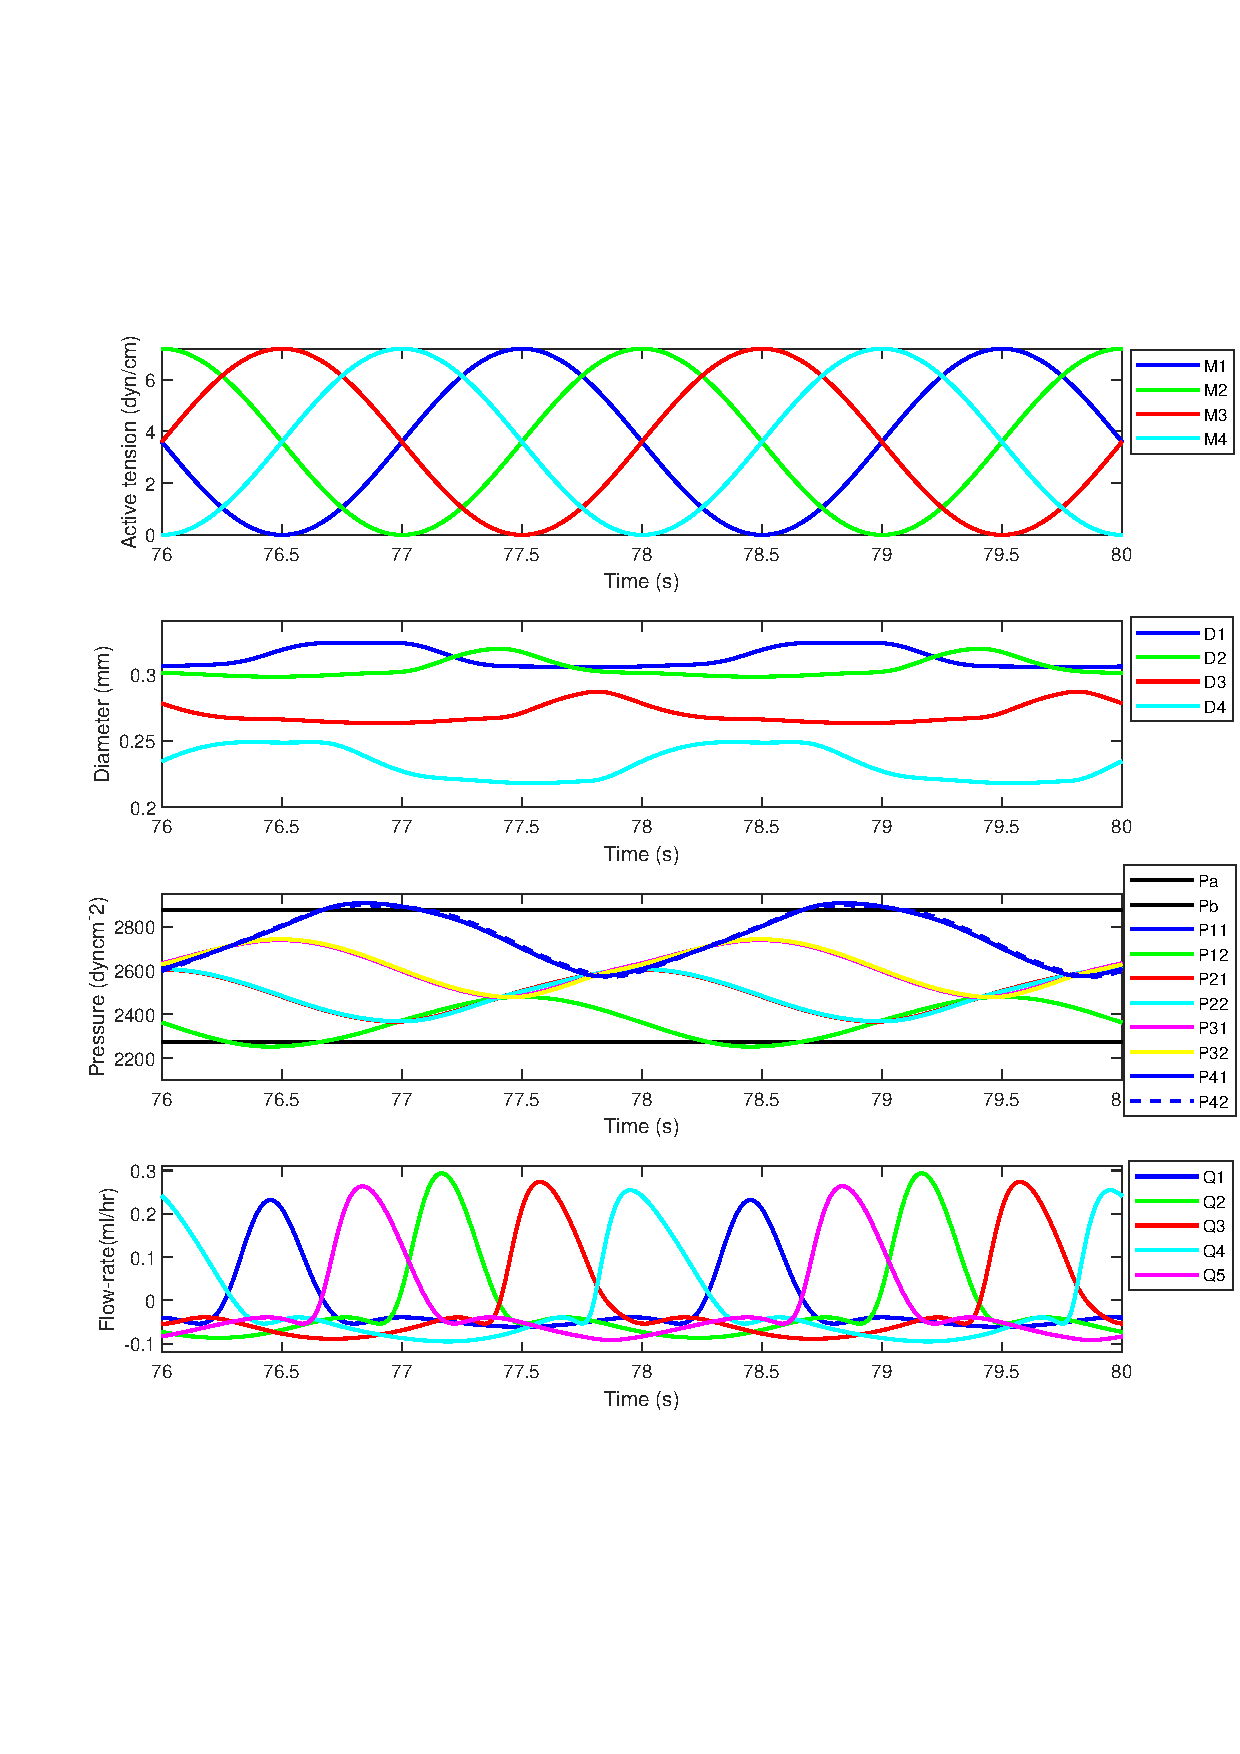
\includegraphics[trim=1.25cm 5.0cm 0.0cm 0.0cm, clip=true, totalheight=0.75\textheight, ]{figure_2_reproduced.pdf}
\caption{Reproduced results corresponding to Figure 4 in the primary paper, demonstrate the cyclic pumping by a sequence of four lymphangions operating against a pressure differential of 600 dyn cm $^{-2}$. The top panel illustrates the active tension waveform in each lymphangion. The second panel displays the dynamic variations in the diameters of the four lymphangions. The third panel presents the eight distinct time-varying pressures, with horizontal black lines denoting the inlet and outlet pressures P$_{a}$ and P$_{b}$. The bottom panel illustrates the flow rate through each of the five valves.}
\label{fig:reproduced_1}
\end{figure}
\begin{figure}[p]\centering
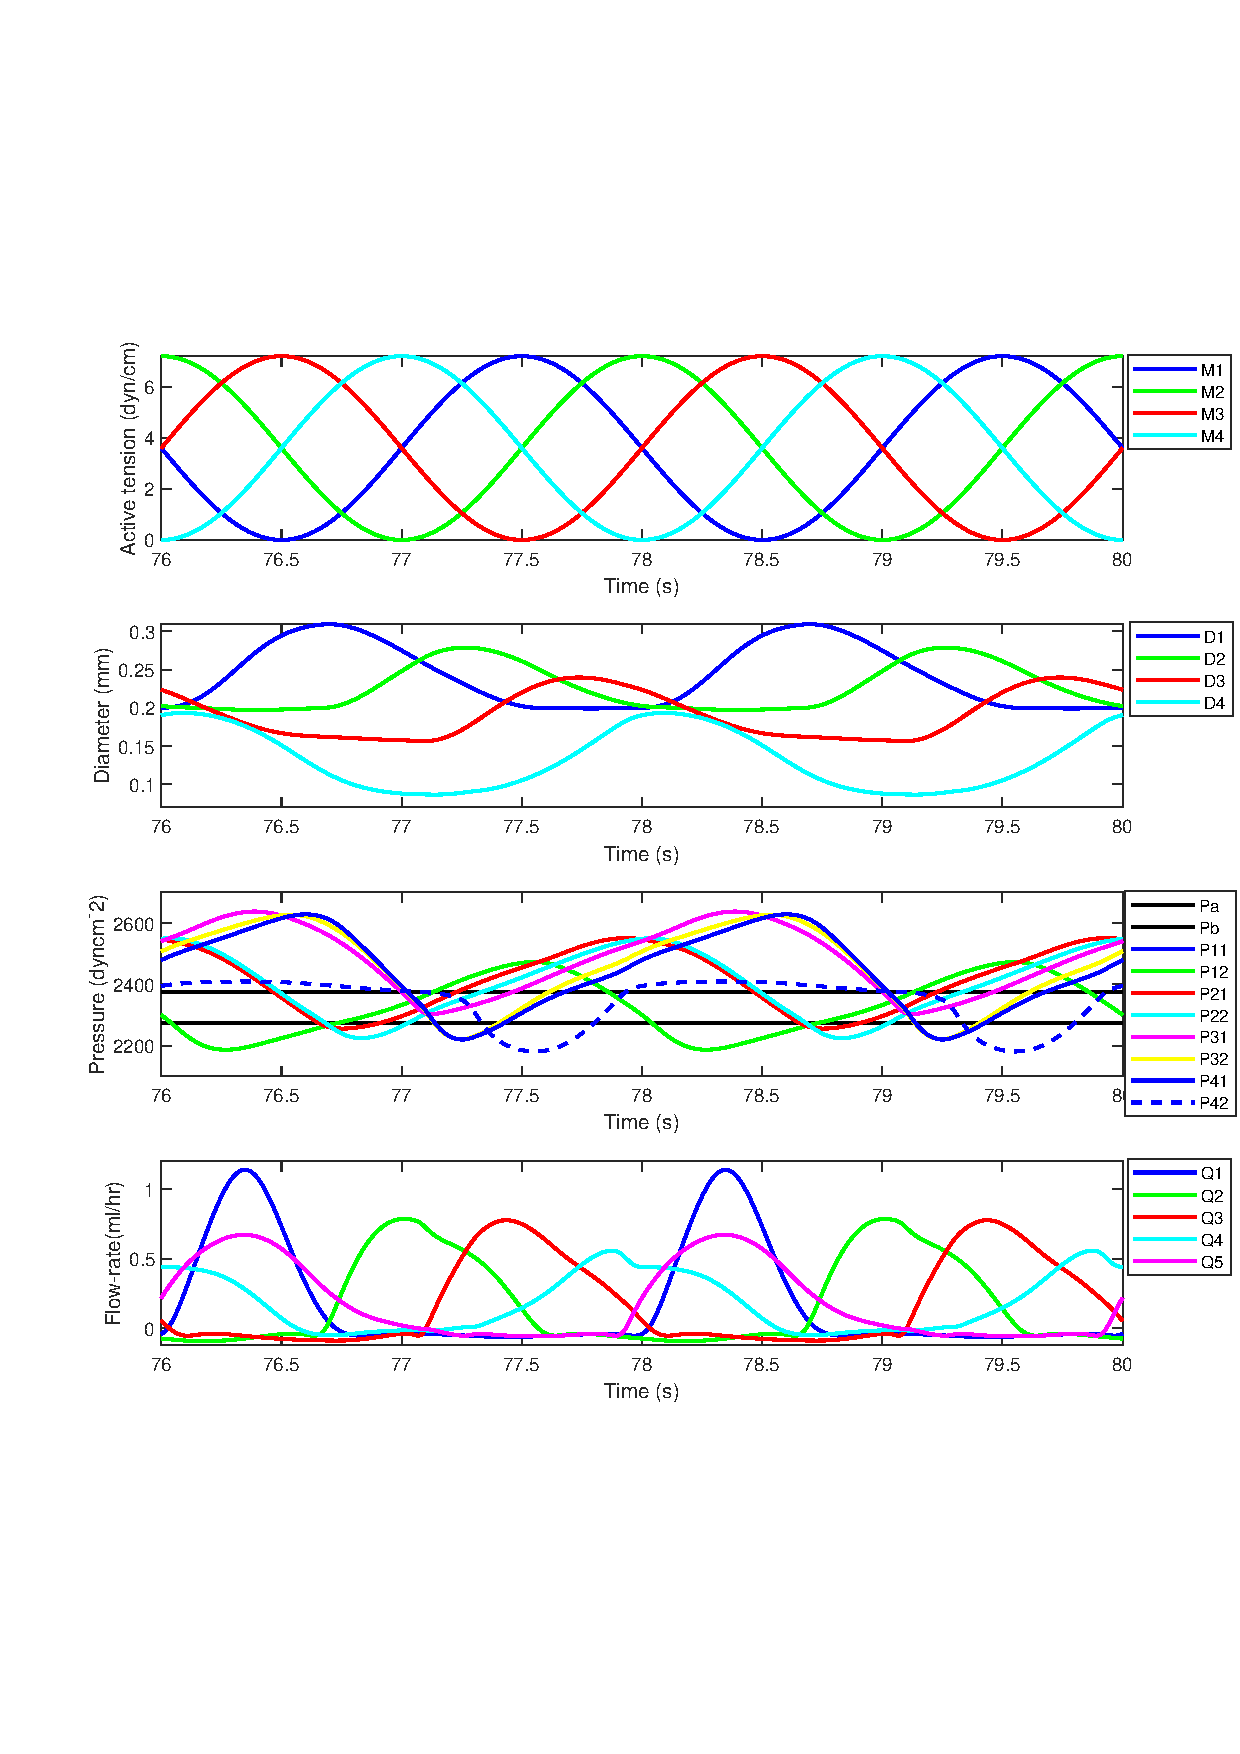
\includegraphics[trim=1.25cm 5.0cm 0.0cm 0.0cm, clip=true, totalheight=0.75\textheight, ]{figure_3_reproduced.pdf}
\caption{Reproduced results corresponding to Figure 5 in the primary paper, demonstrate the cyclic pumping by a sequence of four lymphangions operating against a pressure differential of 100 dyn cm $^{-2}$. The top panel illustrates the active tension waveform in each lymphangion. The second panel displays the dynamic variations in the diameters of the four lymphangions. The third panel presents the eight distinct time-varying pressures, with horizontal black lines denoting the pressures at points P$_{a}$ and P$_{b}$. The bottom panel illustrates the flow rate through each of the five valves.}
\label{fig:reproduced_2}
\end{figure}

\begin{table}[h]
\caption{Parameter values used in the CellML model.}
\label{table_para1}
\begin{center}


\begin{tabular}{|l|l|l|}
\hline
Parameter values    & Figure 4     & Figure 5     \\
\hline
P\_a                & 2275 dyncm$^{-2}$ & 2275 dyncm$^{-2}$ \\
P\_b                & 2875 dyncm$^{-2}$ & 2375 dyncm$^{-2}$ \\
t\_01\_Vessel\_1    & 0.5          & 0.5          \\
P\_d\_01\_Vessel\_1 & 50 dyncm$^{-2}$   & 50 dyncm$^{-2}$   \\
D\_d\_Vessel\_1     & 0.025 cm     & 0.025 cm     \\
t\_01\_Vessel\_2    & 1            & 1            \\
P\_d\_01\_Vessel\_2 & 75 dyncm$^{-2}$   & 75 dyncm$^{-2}$   \\
D\_d\_Vessel\_2     & 0.022cm      & 0.022cm      \\
t\_01\_Vessel\_3    & 1.5          & 1.5          \\
P\_d\_01\_Vessel\_3 & 100 dyncm$^{-2}$  & 100 dyncm$^{-2}$  \\
D\_d\_Vessel\_3     & 0.019 cm     & 0.019 cm     \\
t\_01\_Vessel\_4    & 2            & 2            \\
P\_d\_01\_Vessel\_4 & 125 dyncm$^{-2}$  & 125 dyncm$^{-2}$  \\
D\_d\_Vessel\_4     & 0.016 cm     & 0.016 cm   \\ 
\hline
\end{tabular}
\end{center}
\end{table}
% \section{Discussion}

\newpage

\section{Discussion}
This lymphangion chain model is an efficient computational framework for comprehending the pumping performance and nonlinear dynamics of lymphatic vessel diameter fluctuations. There is no overlap between the authors of the primary paper and our Physiome paper. Our goal was to test the reproducibility of the model originally published by Bertram et al. (2011), independent of the original authors' involvement. Utilizing the reported parameter values, we have effectively replicated and validated the results presented in Figures 4 and 5 of the primary paper. As previously mentioned, subsequent studies have enhanced the intricacy of this model. Consequently, we will be able to curate additional lymphatic models within the PMR, building upon this reproduced model of \cite{bertram2011simulation}.
\section{Acknowledgement}
TDJD was supported in part by a New Zealand Ministry of Business, Innovation and Employment 12 Labours project grant. HMR was supported by a Sir Charles Health Research Fellowship from the Health Research Council of New Zealand grant 20/017. SS acknowledges support from the Aotearoa Foundation. AP and PR were supported in part by Health Research Council of New Zealand grants 20/035 and 21/714.
\bibliography{sample}

\end{document}